% ===== 5. Probing Qwen3-1.7B =====
\section{5. Probing Qwen3-1.7B}\label{probing-qwen3-1.7b}

Before the numbers, the Confabulation Atlas (Figure \ref{fig:atlas},
Appendix A.4) situates them geometrically: a \emph{supervised} 2-D
projection of the layer-18 hidden states of all 784 questions, against
an \emph{unsupervised} PCA(2) control in which PC1+PC2 alone already
support an \(86.9\%\) refusal-vs-wrong probe (vs.~\(73.2\%\) majority),
so the refusal separation is not an artifact of supervised projection.

% ----- 5.1 Accuracy by stratum -----
\subsection{5.1 Accuracy by stratum}\label{accuracy-by-stratum}

Of 784 items, 235 (30.0\%) are graded \texttt{correct}; 147 (18.8\%)
\texttt{refusal}; 402 (51.3\%) \texttt{wrong} (breakdowns in Appendix A,
Table \ref{tbl:bycategory}). The cutoff manipulation works as designed:
pre-cutoff accuracy is 47.3\% (140/296) against 19.5\% (95/488)
post-cutoff, and in the obscure-pre-cutoff cell, the benchmark's
innovation, the model fails on \(\approx 66.7\%\) of items whose answers
existed in its training data, exactly the population the cutoff
disconfound needs. All 147 refusals fall in the post-cutoff cell:
refusal is triggered by the knowledge-cutoff cue rather than intrinsic
uncertainty, motivating the \texttt{refusal\_vs\_wrong\_within\_post}
probe of Section 4.

% ----- 5.2-5.4 Text-level confidence, case studies, geometry -----
\subsection{5.2--5.4 Text-level confidence, confident-confabulation case
studies, and hidden-state geometry}\label{text-level-confidence}

Mean per-token log-probability separates correct from incorrect answers
only in expectation (Figure \ref{fig:confidence}, Appendix A.2):
\(\bar{\ell}_{\mathrm{correct}} \approx -0.10\)
vs.~\(\bar{\ell}_{\mathrm{incorrect}} \approx -0.15\) (\(\approx 0.90\)
vs.~\(\approx 0.86\) geometric-mean per-token probability), with heavy
overlap in \([-0.2, -0.05]\): weakly informative, not a usable
predictor. Table \ref{tbl:topwrong} (Appendix A.3) lists the five
highest-\(\bar\ell\) items per failure label; the five confabulations
all sit at \(\approx 0.95\) geometric-mean per-token probability, and
refusals are paradoxically \emph{high-confidence} text outputs (fluent,
assertive statements of ignorance), so a binary substring grader lumps
both failure modes into one \texttt{incorrect} bucket and text-level
confidence cannot separate them afterward: separating them is what the
three-way judge is for (gold-side validation case study in Appendix
B.2). Unsupervised PCA(2) of the raw hidden state (Figure
\ref{fig:embeddings}, Appendix A.4) shows the classes mixing heavily at
layer 14 while by layer 28 the refusals pull into a distinct cluster
with no supervision, a tight group of confident confabulations
separating out on its own: that late-layer refusal cluster is the
geometry the refusal-vs-wrong probe reads.

% ----- 5.5 Per-layer linear probes against majority baselines -----
\subsection{5.5 Per-layer linear probes against majority
baselines}\label{per-layer-linear-probes-against-majority-baselines}

\begin{figure}
\centering
\pandocbounded{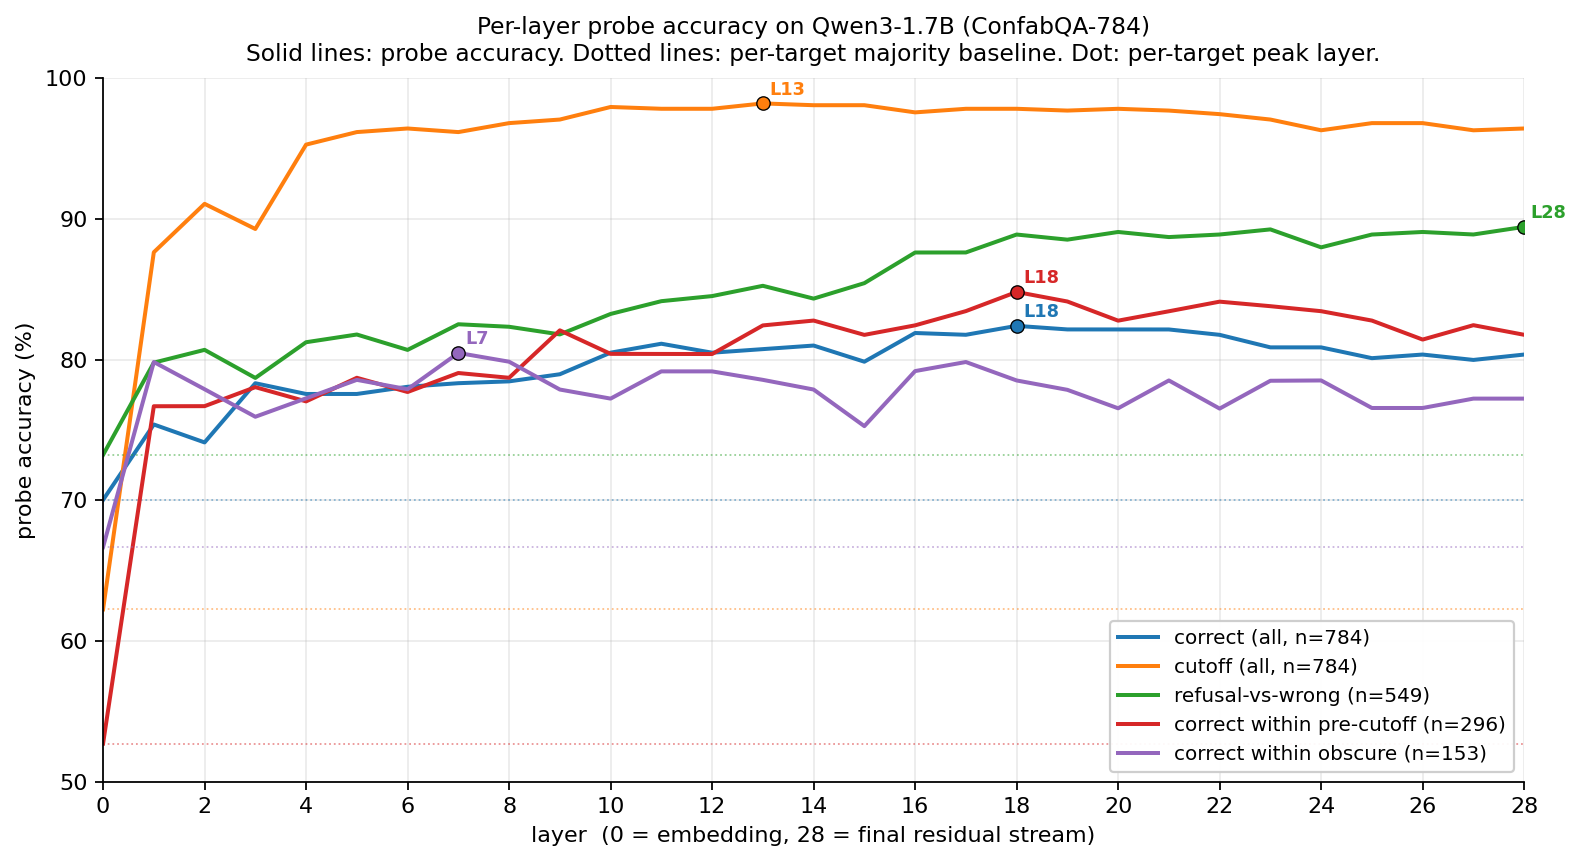
\includegraphics[keepaspectratio,alt={Per-layer probe accuracy for all five
  targets on Qwen3-1.7B (ConfabQA), on a single axis for direct curve-shape comparison.
  Solid lines: probe accuracy per layer. Dotted horizontal lines: per-target majority
  baseline. Dots mark each target's peak layer. Cutoff (orange) saturates near
  98\textbackslash\% by layer 13 and stays high through the network. Refusal-vs-wrong
  (green, n=549) rises monotonically and peaks at the deepest block (layer 28).
  Correctness (blue, n=784) and the cutoff-disconfounded correct-within-pre (red, n=296)
  both peak at layer 18, with within-pre showing the headline +32 pp margin over its
  52.7\textbackslash\% pre-cutoff majority that largely vanishes against the
  prompt-feature baseline of Section 5.6. Correct-within-obscure (purple, n=153) peaks at
  layer 7 but the 1-\textbackslash sigma layer range spans nearly the whole network, so
  the per-layer peak is not statistically pinned at this sample
  size.},width=0.66\linewidth]{figures/per_layer_probes_merged.png}}
\caption{Per-layer probe accuracy for all five targets on Qwen3-1.7B
(ConfabQA). Solid lines: probe accuracy per layer; dotted horizontal
lines: per-target majority baselines; dots: peak layers (values in Table
\ref{tbl:probepeaks}, Appendix A.5). Cutoff saturates early and stays
high; refusal-vs-wrong rises monotonically and peaks at the deepest
block; correctness and correct-within-pre peak mid-network, with
within-pre's headline margin over its pre-cutoff majority largely
vanishing against the prompt-feature baseline of Section 5.6;
correct-within-obscure has a \(1\)-\(\sigma\) layer range spanning
nearly the whole network.}\label{fig:per-layer-probes}
\end{figure}

Table \ref{tbl:probepeaks} (Appendix A.5) tabulates peaks, layer
ranges, and margins over the majority baselines for all five targets,
with the \(1\sigma\) layer-range caveat (the within-obscure range spans
the whole network, so its per-layer peak is not a per-depth claim).
Taken at face value these are the margins a single-model study would
lead with; Section 5.6 explains why every correctness margin among them
is overstated. Imbalance-aware metrics at the refusal-vs-wrong peak
(balanced accuracy \(0.874\), ROC AUC \(0.944\); confusion matrix in
Appendix D.6) show the probe is not defaulting to ``wrong''.

% ----- 5.6 Value of the hidden state compared to prompt features -----
\subsection{5.6 Value of the hidden state compared to prompt
features}\label{value-of-the-hidden-state-compared-to-prompt-features}

Table \ref{tbl:hadds} scores the hidden-state probe against the four
Section 4 baselines on the same folds. The \texttt{+category} baseline
is a \emph{difficulty oracle}: category explains most of the raw
correctness variance by construction (the \(62.2\%/33.3\%/19.5\%\) base
rates of Table \ref{tbl:bycategory}), so scoring against it asks for
item-level signal beyond the coarse difficulty bucket; within
single-category strata the dummy is constant (\texttt{+category}
collapses to \texttt{+domain}), and for \texttt{cutoff} the dummy
\emph{is} the label and is excluded (Section 4).

Full per-target margins over the strongest prompt baseline are in
Table~\ref{tbl:hadds} (Appendix A.5).

(All baselines are 5-fold CV accuracy with \texttt{random\_state=0}.
\(\dagger\): for the \texttt{cutoff} target the category dummy \emph{is}
the label; the tautological \(1.000\) is shown for completeness but
excluded from the strongest-baseline comparison.)

\textbf{Table \ref{tbl:hadds} interpretation.} (1)~\emph{Correctness
gains little from the hidden state}: \(\approx 3\) pp or less over the
strongest baseline (\(+2.4\) pp all items, \(+3.0\) pp within-pre, \(-2.5\) pp
within-obscure), within per-fold noise (\(0.031\)--\(0.063\)); the
Section 8.1 bootstrap confirms the reading (all-items margin real,
disconfounded within-stratum margins consistent with zero).
(2)~\emph{Cutoff is easy to predict either way}: text features alone
reach \(94.0\)--\(95.2\%\) (the year mentioned is a near-perfect
predictor), the probe at \(98.2\%\) adds \(+3.0\) pp; a manipulation
check, not a finding about internals.
(3)~\emph{Refusal-vs-confabulation substantially beats prompt
features}: \(+7.4\) pp over TF-IDF overall, \(+9.6\) pp within
post-cutoff where all refusals occur, gaps \(\approx 4\)x the per-fold
std (\(0.019\), \(0.022\)). The asymmetry is what the targets' nature
predicts: refusal-vs-confabulation is a decision the model itself makes
and the late hidden state is the computation producing it (Section
2.2), so an encoding must exist; correctness is a relation between
output and world, and nothing guarantees the model represents it. What
is not guaranteed, and is the substance of Section 6, is the signal's
form: linearly decodable from \(16\) principal components, concentrated
late, causally sufficient for the first-token opening, and
SAE-decomposable.

